\documentclass{VUMIFPSPraktika}
\usepackage{float}
\usepackage{hyperref}
\usepackage{algorithmicx}
\usepackage{algorithm}
\usepackage{algpseudocode}
\usepackage{amsfonts}
\usepackage{amsmath}
\usepackage{bm}
\usepackage{caption}
\usepackage{color}
\usepackage{graphicx}
\usepackage{listings}
\usepackage{subcaption}
\usepackage{wrapfig}
\usepackage{biblatex}
\usepackage{microtype}
\usepackage{xcolor}
\usepackage{booktabs}
\usepackage{pgfplots}
\usepackage{multirow}
\usepackage{minted}
\usepackage{icomma}
\usepackage{siunitx}
\sisetup{output-decimal-marker={,}}
\pgfplotsset{compat=newest}

\bibliography{bibliografija}

\paper{Praktikos ataskaita}
\author{Pijus Petkevičius}
\title{Mobiliosios programėlės funkcionalumo kūrimas ir tobulinimas}
\englishtitle{Mobile application functionality implementation and refinement}
\department{Programų sistemų bakalauro studijų programa}
\universitysupervisor{Lekt. Irus Grinis}
\organisationsupervisor{\parbox{\linewidth}{\raggedright
Vyr. programinės įrangos inžinierius Vytautas Juozas Barkauskas}}
\date{Vilnius, \the\year}
\begin{document}

\maketitle
\tableofcontents

\sectionnonum{Įvadas}
Pasirinkimą pradėti karjerą \enquote{Bentley Systems} nulėmė įmonės dydis, ilgaamžiškumas ir pagrindinis dėmesys programinės įrangos sprendimams. Šie aspektai buvo svarbūs, nes garantuoja, kad įmonėje kreipiamas dėmesys ne tik į galutinį produktą, bet ir kodavimo standartų, geriausios praktikos laikymąsi. Taip pat įmonės dydis garantuoja, kad joje dirbantys darbuotojai yra patyrę, savo srities ekspertai, kurie padės išspręsti iškilusias problemas ir įgyti darbo su dideliu produktu, darbo komandoje patirties. Įmonė didelį dėmesį skiria ir naujų profesionalų parengimui. Gerai pasirodę praktikantai, kviečiami dalyvauti 2 metų rotacijos programoje, kur kiekvienos rotacijos metu inžinieriai skatinami pasirinkti įvairias programavimo technologijas, siekiant rasti jam labiausiai patikusią komandą ir sritį.
Kiekviena rotacija šiose komandose trunka pusmetį ir programuotojams leidžia  susipažinti įmonės įvairiais produktais, komandos nariais. Baigus šias rotacijas, programuotojas gali pasirinkti iš komandų, kurioje toliau tęs savo karjerą.
\bigskip

Šios praktikos \textbf{tikslas} - mobiliosios programėlės funkcionalumo kūrimas ir tobulinimas.
\bigskip

Šios praktikos \textbf{uždaviniai}:
\begin{enumerate}
    \item Pagilinti Kotlin programavimo kalbos žinias rašant programinį kodą.
    \item Išmokti naudotis “Jetpack Compose” Android įrankių rinkiniu skirtu kurti vartotojo sąsają.
    \item Susipažinti su lanksčiojo programavimo projektų valdymo metodu “Kanban”.
    \item Susipažinti su švaraus ir kokybiško kodo rašymo principais ir geriausiomis praktikomis. 
    \item Įgyvendinti naują funkcionalumą Android programėlėje.
\end{enumerate}
\bigskip

Praktika truko 10-11 savaičių, ją atlikau 2024-02-05 -- 2022-04-15.
\bigskip
Šio darbo pirmajame skyriuje aprašoma įmonė \enquote{Bentley systems}, jos veiklos sritis, organizacinė struktūra ir sudarytos darbo sąlygos. Antrajame skyriuje aprašoma praktikos veikla -- tai, kokia buvo užduotis ir kaip ji įgyvendinta. Trečiajame skyriuje pateikiami praktikos darbo rezultatai ir išvados, privalumai ir trūkumai, įgytos žinios bei rekomendacijos universitetui ir organizacijai.


\section{Įmonės apibūdinimas}
Šiame skyriuje aprašoma įmonė \enquote{Bentley systems}, jos veiklos sritis, organizacinė struktūra ir sudarytos darbo sąlygos.
\subsection{Įmonės veiklos sritis}


\enquote{Bentley Systems} yra inovatyvi, pasaulinė programinės įrangos sprendimų, pritaikytų inžinerijos, architektūros, statybos ir infrastruktūros sektoriams, įmonė. Įmonė įkurta 1984 m. amerikiečių brolių Bentley'ų, šiuo metu bendrovė išsiplėtusi į 50 šalių. Lietuvoje filialas „Bentley Systems Europe B.V“ atidarytas 2005 metais. 2015 metais įmonė išsiplėtė Lietuvoje ir buvo atidarytas antras filialas Kaune. Ši įmonė kuria įvairias su modeliavimu susijusias programas (\emph{angl. CAD Modeling and Visualization}) kaip AssetWise, ProjectWise MicroStation, taip pat ir skaitmeninių dvynių (\emph{angl. digital twins}) technologijas, skirtas realaus pasaulio objektų ir procesų virtualiems atvaizdams kurti. Skaitmeniniai dvyniai padeda geriau suprasti, valdyti ir optimizuoti infrastruktūros projektus, taip pat pagerinti jų efektyvumą ir tvarumą.

\subsection{Įmonės organizacinė struktūra}
Šiuo metu organizacija turi daugiau nei 250 pilnu etatu dirbančių darbuotojų Lietuvoje, taip pat įmonė įsikūrusi JAV, Kanadoje, Brazilijoje, Australijoje ir kitose šalyse. Organizacija yra projektinės struktūros - siūlomos įvairios paslaugos, kurių kūrimui ir tobulinimui yra atsakingos komandos įvairiose šalyse, dirbančios pagal Scrum ar Kanban projektų valdymo metodą. Lietuvoje esančios komandos yra tarptautinės, turinčios darbuotojų užsienio šalyse. Komandas dažniausiai sudaro programuotojai, testuotojai, dizaineriai.

\subsection{Įmonės sudarytos darbo sąlygos}
\enquote{Bentley systems} suteikia galimybę dirbti prie didelės kodo bazės projektų. Gavus praktikos vietą, praktikantas yra priskiriamas 3 mėnesiams dirbti prie vieno projekto pilnu etatu (jei dirbama pusę etato - praktika trunka 6 mėnesius). \enquote{Bentley systems} suteikia galimybę dirbti prie įvairių technologijų. Gavus darbo vietą prie \textit{frontend} projekto, dažniausiai naudojama React programavimo karkasas kartu su TypeScript programavimo kalba, \textit{backend}, projektai parašyti C++ ir C\# programavimo kalbomis, kuriant mobiliasias programėles, naudojama Kotlin ir Swift programavimo kalbos Android ir iOS prietaisams. Pateikti paraiškas dėl praktikos vietos galima bet kuriuo metu, dažniausiai praktikantai ieškomi Vasario, Gegužės mėnesiais.

Kiekvienam praktikantui priskiriamas mentorius, dirbantis prie praktikantui priskirto projekto. Mentorius užima aukštesnę nei jaunesniojo programuotojo poziciją. Mentorius padėdavo kilus klausimams, peržiūrėjo programinio kodo pakeitimus, pateikdavo pasiūlymus, kaip galima toliau tobulėti.

Praktika buvo vykdoma hibridiniu būdu - darbas iš ofiso nėra privalomas, tačiau norint gauti, kaip galima greičiau, atsakymus į savo klausimus, rekomenduojama ateiti į ofisą. Kiekvieną trečiadienį komanda susirenka ofise, tad yra puiki galimybė susipažinti su savo komandos nariais. Ofisas įsikūręs adresu Švitrigailos g. 13.

Praktikos metu įmonė suteikė kompiuterinę įrangą praktikantams, reikalingas licencijas norint pradėti darbuotis su nauju projektu. Praktikos metu buvo kompensuotas komandos susitikimo renginys (\emph{angl. Team building}). Ofise praktikantui yra priskiriama komandos kabinete esanti vieta, norint dirbti iš ofiso. \enquote{Bentley systems} įmonėje atlikta praktika buvo apmokama.
\section{Praktikos veiklos aprašymas}
Šį skyrių sudaro praktikos veiklos aprašymas ir jos įgyvendinimas.

\subsection{Praktikos vietos gavimas}
Norint gauti praktikos vietą \enquote{Bentley systems} reikėjo atlikti 3 su programavimu susijusias užduotis \enquote{Codility} aplinkoje. Jei šios užduotys buvo atliktos gerai, kandidatas kviečiamas antram etapui. Antrojo etapo metu \enquote{Codility} aplinkoje susipažinama su programuotojais, kurie stebės kandidato užduočių atlikimą, padės jei iškils problemų. Prieš pradedant atlikti naujas užduotis, diskutuojamos pirmo etapo užduotys, kas galėjo būti geriau, kodėl tam tikri kodo sprendimai buvo priimti. Po diskusijos pateikiamos pora užduočių, kandidatas bando jas išspręsti, užstrigus, programuotojai padeda. Užduotys olimpiadinio programavimo pobūdžio ir objektinio programavimo pagrindų patikrinimo.

Pirmoji darbo diena prasidėjo nuo terminuotos sutarties pasirašymo. Po to supažindino su komanda, mentoriumi, su kuriuo dirbsiu artimiausius 3 mėnesius. Komandą sudaro 15 narių: 3 testuotojai, 1 projektų vadovas ir 12 įvairaus lygio programuotojų. Kas 3 savaites susitinkama su mentoriumi pasidalinti su per 3 savaites įvykusiais įvykiais, atsiradusiomis problemomis, diskutuojama kaip jos galėtų būti išspręstos.

% Praktikos veiklos aprašymas (vienas arba keli skyriai). Aprašomas praktikos užduoties įgyvendinimas (pvz., atlikti projektavimo ir/ar programavimo darbai, sukurtas modelis, priimti sprendimai ir pan.).
\subsection{Praktikos užduotys}

Šiame poskyryje pateiktos visos užduotys, kurios buvo atliktos praktikos metu. Kiekviena užduotis bus trumpai apibūdinta, įvardinant jos tikslą, įgyvendinimo būdus ir pasiektus rezultatus mobiliojoje programėlėje.

\subsubsection{Tap to fullscreen on iOS}

Ši užduotis buvo skirta realizuoti programos lango pakeitimą į pilno ekrano režimą spustelėjus ant tuščios dokumente vietos, Pdf peržiūros lange. Užduotis buvo paskirstyta į 2 dalis: Android ir iOS. Pasirinkau realizuoti funkcionalumą iOS prietaisuose.

Reikalavimai atliekant užduotį:

\begin{enumerate}
    \item PdfTron anotacijų sąrašas:
    \begin{enumerate}
        \item Komponentų paslėpimas: \enquote{PdfTron}, \enquote{Synchro field} navigacijos, statuso juosta ir apatinė anotacijų juosta turėtų būti paslėpti, kai pdf ekranas apima visą ekraną.
        \item Pdf užimti visą ekraną ir sugrįžti atgal į normalią būseną.
    \end{enumerate}
    \item Kai anotacijų sąrašas atidarytas(telefone):
    \begin{enumerate}
        \item Turėtų elgtis taip pat, tik anotacijų sąrašas turi irgi dingti, kai Pdf ekranas užima visą ekraną.
    \end{enumerate}
    \item Kai anotacijų sąrašas atidarytas(plančetiniame):
    \begin{enumerate}
        \item Turėtų elgtis taip pat, tik šoninio anotacijų sąrašo neuždaryti.
    \end{enumerate}
\end{enumerate}


\enquote{Synchro Field} projekte norint peržiūrėti Pdf failus naudojame biblioteką \enquote{PdfTron} (\ref{fig:pdfViewController screen} paveikslėlis). Tačiau, \enquote{PdfTron} komponento navigacijos juosta yra atskirta nuo \enquote{Synchro field} navigacijos juostos (\ref{img:pdfViewController} paveikslėlis). Reikėjo pridėti pakeitimus funkcijai, kuri įvykdoma, kai \enquote{PdfTron} navigacijos juostos matomumas pasikeičia. \ref{fig:pdfTronCode} paveikslėlyje galime matyti, kad funkcijai pradėjus vykdymą, naudojama \textit{UIView.animate()} funkcija, kuri sklandžiai suanimuoja vartotojo sąsajos pasikeitimus. Patikrinama ar naujas funkcionalumas yra įjungtas su \enquote{feature flag}. Atliekami \enquote{Synchro field} navigacijos juostos apribojimų reikšmių pakeitimai. Animacijos trukmė parinkta 0,2 sekundės, siekiant sulyginti \enquote{PdfTron} ir \enquote{Synchro field} navigacijos laukų animacijų trukmes. Jei anotacijų sąrašas yra atidarytas (\ref{img:annotationList} paveikslėlis), sąrašas paslepiamas.

Šio funkcionalumo programavimo metu teko ne tik rašyti kodą, bet ir išmokti naudotis \enquote{Storyboards}. \enquote{PdfTron} lange reikėjo pridėti papildomų apribojimų (\emph{angl. constraints}), siekiant padidinti Pdf komponento dydį.


\begin{figure}[htbp!]
    \centering
\begin{minted}[linenos,tabsize=1,breaklines]{swift}
extension PdfTronViewController: PdfTronNavigationControllerDelegate {
    func pdfTronNavigationController(didSetNavigationBarHidden isHidden: Bool) {
        UIView.animate(withDuration: 0.2) { [weak self] in
            guard let self else { return }
            if Features.isEnabled(DevelopmentFeatureFlag.pdfMarkupNative) {
                labeledBottomBarHeightConstraint.isActive = isHidden
            }
            setNavigationBarVisibility(isHidden)
            view.layoutIfNeeded()
        }

        if let resizablePanelViewController, resizablePanelViewController.panelStatus != .closed {
            resizablePanelViewController.shouldResize = !isHidden
            let panelHeight = isHidden ? 0 : resizablePanelViewController.heightHalfExpanded
            resizablePanelViewController.animatePanelToHeight(panelHeight)
        }
    }

    private func setNavigationBarVisibility(_ isHidden: Bool) {
        setStatusBarHidden(isHidden)
        if Features.isEnabled(DevelopmentFeatureFlag.pdfMarkupNative) {
            navigationBarTopConstraint.isActive = isHidden
            navigationBarSafeAreaTopConstraint.isActive = !isHidden
            navigationBarShowingConstraint.constant = isHidden ? 0 : navigationBarHeight
        }
    }
}
\end{minted}
\caption{PdfTronViewController matomumo kodas}
    \label{fig:pdfTronCode}
\end{figure}


    
\subsubsection{UIButton configuration}
Ši užduotis buvo skirta perkelti didžiąją dalį mygtukų iOS projekte į FieldUIComponents projektą ir su vienodinti stilių nustatymą naudojant \enquote{UIButton.Configuration}.

Reikalavimai atliekant užduotį:
\begin{enumerate}
    \item Perkelti mygtuko vartotojo sąsajos kodą į FieldUIComponents projektą.
    \item Atnaujinti Field projekto kodo bazę su naujais mygtukų komponentais.
    \item Vizualių pakeitimų neturi būti.
\end{enumerate}

Pirmiausia buvo pereita per visą projektą, pažymėtos vietos, klasių mygtukai, kurie galėtų būti perkelti į FieldUIComponents projektą. Perkėlus mygtukus, pradėta perrašyti mygtukų stiliaus nustatymas su \enquote{UIButton.Configuration} (\ref{fig:Primary button} paveikslėlis). Teksto spalvos, šrifto ir dydžio nustatymas negalėjo būti perrašytas \enquote{UIButton.Configuration} pagalba, nes pakeitus mygtuko tekstą, reikšmės įgavo pradines stiliaus reikšmes. 

\begin{figure}[htbp!]
    \centering
    \begin{minted}[linenos,tabsize=1,breaklines]{swift}
@IBDesignable public class PrimaryButton: BaseUIButton {
    override func sharedInit() {
        var configuration = UIButton.Configuration.plain()
        configuration.background.cornerRadius = 3
        configuration.background.backgroundColor = UIColor(fieldColor: .blueCerulean)
        configuration.titleLineBreakMode = .byTruncatingMiddle
        self.configuration = configuration
        setAttributedTitle(font: UIFont.openSans(ofSize: 14), foregroundColor: UIColor(fieldColor: .white))
    }
    ...
}
    \end{minted}
    \caption{Primary button kodo perrašymas naudojant UIButton.Configuration}
    \label{fig:Primary button}
\end{figure}


Taip pat buvo sukurtas FieldUIComponentsApp langas, kuriame galima rasti visus projekte naudojamus mygtukus (\ref{fig:buttonsView.png} paveikslėlis). Kadangi mygtukų langas parašytas su SwiftUI, o patys mygtukai su UIKit funckijomis, reikėjo sukurti\textit{ButtonViewRepresentable}, kuris pasirinktą UIView komponento klasė supakuojama į SwiftUI komponentą, realizavus \textit{UIViewRepresentable} klasės funkcijas (\ref{fig:buttonViewRepresentable} paveikslėlis).

\begin{figure} [htbp!]
    \centering
    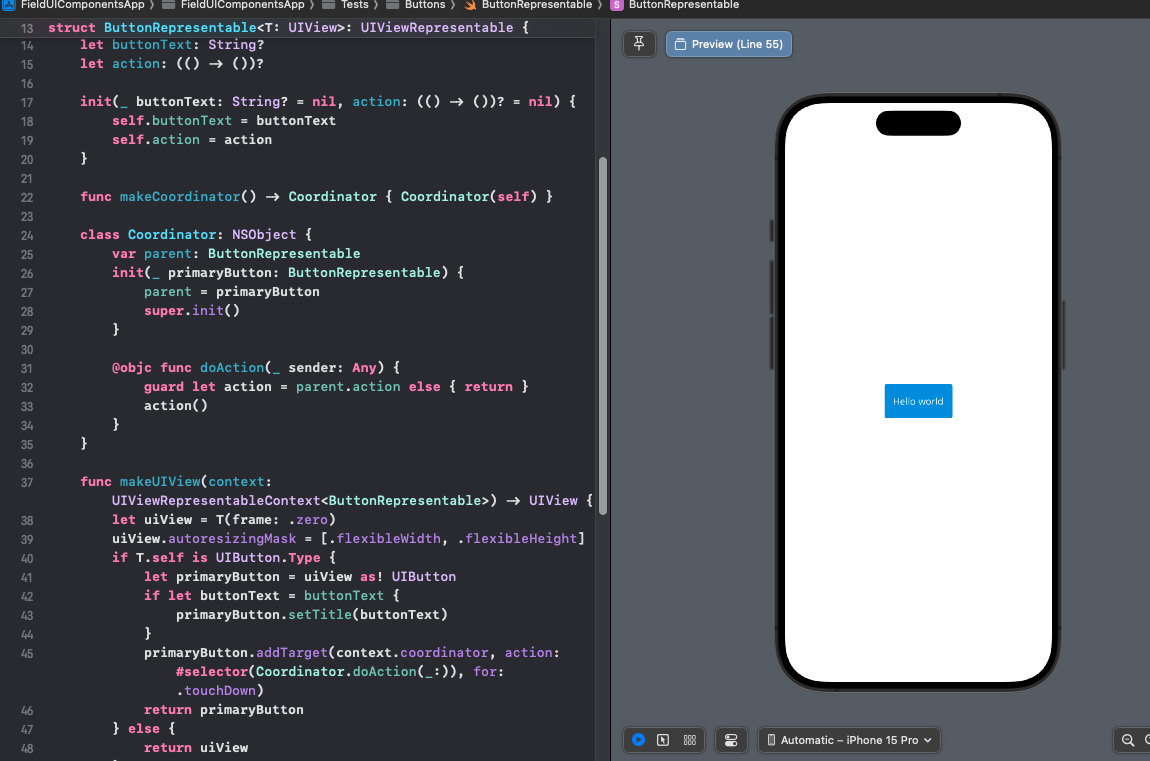
\includegraphics[width=1\textwidth]{Images/iOSButtonRepresentable.png}
    \caption{ButtonViewRepresentable failas}
    \label{fig:buttonViewRepresentable}
\end{figure}

\newpage
\subsubsection{Custom Toast message on Android}
Ši užduotis buvo skirta realizuoti UX sukurtą iššokančių žinučių (\emph{angl. Toast messages}) komponentą Android ir iOS operacinėse sistemose. 
Buvo sukurti FieldUIComponents app langai, kuriuose galima įvairiais būdais ištestuoti iššokančias žinutes.

Pasirinkau atlikti šią užduotį Android prietaisuose. 

Reikalavimai atliekant užduotį:
\begin{enumerate}
    \item Sukurti padengtą testais FieldUIComponents komponentą.
    \item Sukurti naują iššokančių žinučių komponentą.
    \begin{enumerate}
        \item Teksto žinutė
        \begin{enumerate}
            \item Tekstas turi tilpti į vieną eilutę.
            \item Jei tekstas užima daugiau vietos, sutrumpinti su \enquote{...}.
            \item Komponento animacija turi kiek galima daugiau sutapti su maketo animacijomis.
        \end{enumerate}
        \item Iššokančios žinutės animacijos trukmė - 3 sekundės.
        \item Iššokanti žinutė galima paslėpti paspaudus ant jos ar atlikus tempimo į viršų gestą.
    \end{enumerate}
    \item Iššokančių žinučių eilė:
    \begin{enumerate}
        \item Iššokančios žinutės patenka į eilę, rodomos viena po kitos, paslepiamos tokia pačia tvarka kaip ir buvo parodytos.
        \item Tokios pačios žinutės nerodomos 2 kartus.
    \end{enumerate}
\end{enumerate}
\newpage
Iš pradžių buvo sukurtas iššokančios žinutės komponentas (\ref{fig:pill} paveikslėlis). Komponentui pritaikytos gestų atpažinimo, paspaudimo funkcionalumas, teksto sutrumpinimas (\ref{fig:pillCode} paveikslėlis).

\begin{figure}[htbp!]
    \centering
    \begin{minted}[linenos,tabsize=1,breaklines]{kotlin}
@Composable
fun Pill(
    modifier: Modifier = Modifier,
    text: String,
    fontSize: TextUnit = dimensionResource(id = R.dimen.toast_font_size).value.sp,
    horizontalPadding: Dp = dimensionResource(id = R.dimen.toast_padding_horizontal),
    verticalPadding: Dp = dimensionResource(id = R.dimen.toast_padding_vertical)
) {
    Surface(
        modifier = modifier
            .padding(horizontal = horizontalPadding),
        shape = CircleShape,
        color = colorResource(R.color.toastBackground)
    ) {
        Row(
            modifier = Modifier
                .wrapContentWidth()
                .padding(horizontalPadding, verticalPadding),
            horizontalArrangement = Arrangement.Center
        ) {
            Text(
                text = text,
                textAlign = TextAlign.Center,
                fontSize = fontSize,
                color = Color.White,
                style = MaterialTheme.typography.body2,
                maxLines = 1,
                overflow = TextOverflow.Ellipsis
            )
        }
    }
}
    \end{minted}
    \caption{Iššokančios žinutės komponento kodas}
    \label{fig:pillCode}
\end{figure}
\newpage
Sukurtas \enquote{ToastViewModel}, kuris rūpinasi iššokančių žinučių eile, patikrina eilėje esančias žinutes, jei eilėje egzistuoja žinutė, antrą kartą jos neparodys (\ref{fig:ToastViewModel} paveikslėlis). Taip pat galima pateikti žinutės trukmę. pasibaigus trukmei, žinutė išmetama iš eilės.

\begin{figure}[htbp!]
    \centering
    \begin{minted}[linenos,tabsize=1,breaklines]{kotlin}
class ToastViewModel : ViewModel() {
    private val _toastDataState = MutableStateFlow<ToastData?>(null)
    val toastDataState = _toastDataState.asStateFlow()

    private val mutex = Mutex()

    private var pendingMessages: MutableSet<String> = mutableSetOf()

    fun showToast(
        message: String,
        duration: Long = 3000L
    ) {
        if (pendingMessages.isEmpty() || pendingMessages.last() != message) {
            pendingMessages.add(message)
            viewModelScope.launchSafe {
                mutex.withLock {
                    try {
                        return@launchSafe suspendCancellableCoroutine { continuation ->
                            _toastDataState.value = ToastData(message, duration, continuation)
                        }
                    } finally {
                        _toastDataState.value = null
                        pendingMessages.remove(message)
                    }
                }
            }
        }
    }
}
    \end{minted}
    \caption{ToastViewModel programinis kodas}
    \label{fig:ToastViewModel}
\end{figure}

\newpage
Buvo sukurtas \enquote{ToastHost}, skirtas tvarkingai, su animacijomis parodyti iššokančias žinutes  (\ref{fig:ToastHost} paveikslėlis). Panaudota 1,5 konstanta, kad paslėpti iššokančią žinutę, kai kyla į viršų už navigacijos juostos. Standumo ir kiti animacijos parametrai parinkti, kad kuo labiau atitiktų Figma maketų animacijas.

\begin{figure}[htbp!]
    \centering
    \begin{minted}[linenos,tabsize=1,breaklines]{kotlin}
...
val animationOffset: (Int) -> Int = { (heightToDropPx + it * 1.5).toInt() * -1 }
val springAnimationSpec: FiniteAnimationSpec<IntOffset> = spring(
    dampingRatio = Spring.DampingRatioMediumBouncy,
    stiffness = Spring.StiffnessMedium
)

LaunchedEffect(currentToastData) {
    setVisibility(true)
    delay(currentToastData.duration)
    setVisibility(false)
}

AnimatedVisibility(
    modifier = modifier.padding(top = heightToDrop),
    enter = slideInVertically(springAnimationSpec, initialOffsetY = animationOffset),
    exit = slideOutVertically(springAnimationSpec, targetOffsetY = animationOffset),
    visibleState = isVisible,
    content = { toast() }
)
...
    \end{minted}
    \caption{ToastHost programinis kodas}
    \label{fig:ToastHost}
\end{figure}

\newpage
Kadangi \enquote{Jetpack Compose} komponentų tiesiogiai integruoti į fragmentais pagrįstą programėlę, reikėjo sukurti papildomą klasę \enquote{Toasts} (\ref{fig:Toasts} paveikslėlis). Jame padavus tėvinį vaizdą (\emph{angl. root view}) programiniu būdu prideda \enquote{Jetpack Compose} komponentą. Kadangi programėlė yra suprogramuota naudojantis daug fragmentų ir 1 \textit{activity}, iššokančios žinutės matysis visoje programėlėje. Galutinį rezultatą galima matyti \ref{fig:modelToastView} paveikslėlyje.

\begin{figure}[htbp!]
    \centering
    \begin{minted}[linenos,tabsize=1,breaklines]{kotlin}
class Toasts(private val context: Context) {
    private var view: View? = null
    fun addToastView(activityRootLayout: ViewGroup?) {
        val rootView = activityRootLayout ?: return
        if (view == null)
            createToastView(rootView)
    }

    private fun createToastView(rootView: ViewGroup) {
        val view = ComposeView(context).apply {
        setViewCompositionStrategy(ViewCompositionStrategy.DisposeOnViewTreeLifecycleDestroyed)
            setContent {
                Column {
                    Toast(toastViewModel = toastViewModel)
                }
            }
        }

        this.view = view
        rootView.addView(view)
        rootView.bringChildToFront(view)
        view.requestLayout()
    }
}
\end{minted}
    \caption{Toasts komponentas}
    \label{fig:Toasts}
\end{figure}

\section{Rezultatai, išvados ir pasiūlymai}

\textbf{Praktikos darbo privalumai}:
\begin{enumerate}
    \item Taikomos naujos technologijos.
    \item Galimybė laisvai rinktis norimas užduotis.
    \item Draugiška, padedanti komanda.
\end{enumerate}
\bigskip

\textbf{Praktikos darbo trūkumai}:
\begin{enumerate}
    \item Praktikantai dažnai jaučiasi izoliuoti vienoje komandoje, baugu susipažinti su kitais praktikantais, praktikantų susitikimai nuotoliniai, kas pasunkina socializacijos aspektą.
\end{enumerate}
\bigskip

\textbf{Įgytos žinios ir patirtis praktikos metu:}
\begin{enumerate}
    \item Įgyta patirties rašant programinį kodą Kotlin programavimo kalba.
    \item Įgyta žinių apie “Jetpack Compose” Android įrankių rinkiniu skirtu kurti vartotojo sąsają.
    \item Lavinau darbo komandoje gebėjimus ir darbo \enquote{Kanban} projektų valdymo metodo pagalba.
    \item Įgyta patirties rašant kodą su švaraus ir kokybiško rašymo principais ir geriausiomis praktikomis. 
    \item Įgyvendintas naujas funkcionalumas Android programėlėje.
\end{enumerate}
\bigskip

\textbf{Pasiūlymai įmonei}:
\begin{enumerate}
    \item Įmonėje, šiuo metu, į praktikos pozicijas priimami tik programuotojai ir testuotojai. Būtų galima išplėsti praktikos pozicijų pasirinkimą, pridedant projektų vadovo, vartotojo sąsajos dizainerių pozicijas.
    \item Atliekant praktiką, neteko susidurti su realių programinės įrangos, funkcionalumų įvertinimo iš vartotojų pusės. Bet 2,5 mėnesių, manau, yra per mažas laiko tarpas, kad įgyvendintas funkcionalumas pasiektų vartotojus.
    \item Pirmą kartą pamačius projektą, buvo nelabai aišku, koks jo pilnas funkcionalumas, didžiąją dalį funkcionalumo atradau atlikdamas programinio kodo pakeitimus. Galima praktikantams, prieš pradedant rašyti kodą, pristatyti projekto funkcionalumą.
\end{enumerate}
% \begin{enumerate}
%     % \item Grupinių projektinių darbų pristatymų metu per daug skiriama dėmesio sistemos funkcionalumui ir pristatymo sklandumui. Dėl to dažniausiai nukenčia sistemos testavimas -- jaunieji programuotojai nerašo testų, kadangi tai nėra vertinama pristatymo metu.
% \end{enumerate}


\textbf{Pasiūlymai universitetui}
\begin{enumerate}
    \item Praktikos metu teko dirbti prie mobiliųjų programėlių, jų funkcionalumo tobulinimo, universitete, mano žiniomis, privalomojo ar pasirenkamojo dalyko programų sistemų programoje nėra, tad būtų pravartu turėti bent vieną kursą, kuris leistų susipažinti ne tik su interneto svetainių kūrimu, bet ir su kitokia programų kūrimo paradigma.
    \item Galimybė dirbti prie žymiai didesnio projekto. Paskaitų metu, dažniausiai dirbama prie nuo nulio kuriamų projektų, tačiau darbas prie didelės kodo bazės, kurios ankščiau studentas nematė, būtų naudinga patirtis, nes atėjus į darbovietę, studentas, dažniausiai negaus kurti projekto nuo nulio ir teks dirbti prie senesnio, ne su visomis geriausiomis programavimo praktikomis.
    \item Pridėti vartotojo sąsajos testavimo modulį. Universitete testavimo kurse, buvo kalbama apie vienetinius, integracinius, prasiskverbimo testus, apie vartoto sąsają nebuvo užsiminta. Būtų galima supažindinti studentus su pagrindiniais mobiliųjų programėlių testavimo būdais, nes didžiąją dalį vartotojo sąsajos testavimo žinių įgavau tik praktikos metu. 
\end{enumerate}

\setcounter{figure}{0}

\renewcommand{\thefigure}{\alph{figure}}

\section{Priedai}
\subsection{Mobiliosios programėlės komponentų apribojimai lange}
Programuojant mobiliųjų programėlių langus, itin svarbu matyti visus komponentų apribojimus (\emph{angl. constraints}), išdėstymą, kaip kiekvienas komponentas susijungęs vienas su kitu.
Kiekvienas apribojimas gali būti skirtingas įvairiems mobiliųjų prietaisų ekranams, prietaiso orientacijai. Visi apribojimai Storyboards karkase aprašomi naudojant XML kalbą. SwiftUI atveju, kiekvienas specifinis atvejis aprašomas Swift kalba. Asmeniškai, SwiftUI komponentų aprašymas itin panašus į Jetpack Compose, yra lengvai suprantamas, lyginant su Android ir iOS XML komponentų aprašymu.
\begin{figure}[htbp!]
    \centering
    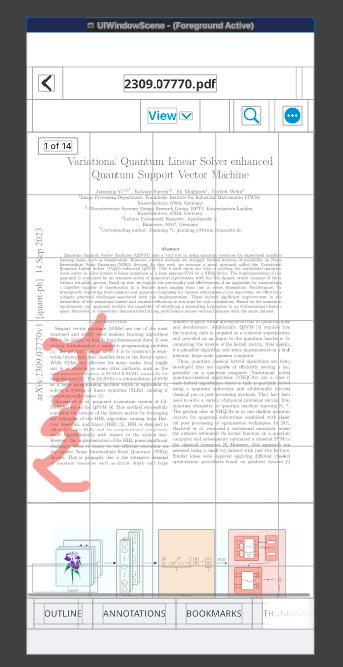
\includegraphics[width=0.5\textwidth]{Images/PdfTronViewController.png}
    \caption{PdfTronViewController ekranas}
    \label{fig:pdfViewController screen}
\end{figure}
\newpage
\subsection{Mobiliosios programėlės komponentų išskaidymas}

Programuojant mobiliasias progamėles, itin naudinga matyti, kokie komponentai buvo naudojami specifiniame mobiliosios programėlės lange. Tai leidžia greitai ir efektyviai identifikuoti, kurie komponentai yra naudojami ir kaip jie yra sukonfigūruoti.
\ref{img:pdfViewController} paveikslėlyje galime matyti, kaip atrodo \enquote{PdfTronView} dekompozicija, ekraną galima pasukti, norint pamatyti 3d dekompoziciją. Ieškant iškilusių problemų dideliame projekte, šis funkcionalumas yra labai naudingas, nes leidžia greitai rasti kokie komponentai naudojami, jų pavadinimus. 
\begin{figure}[htbp!]
    \centering
    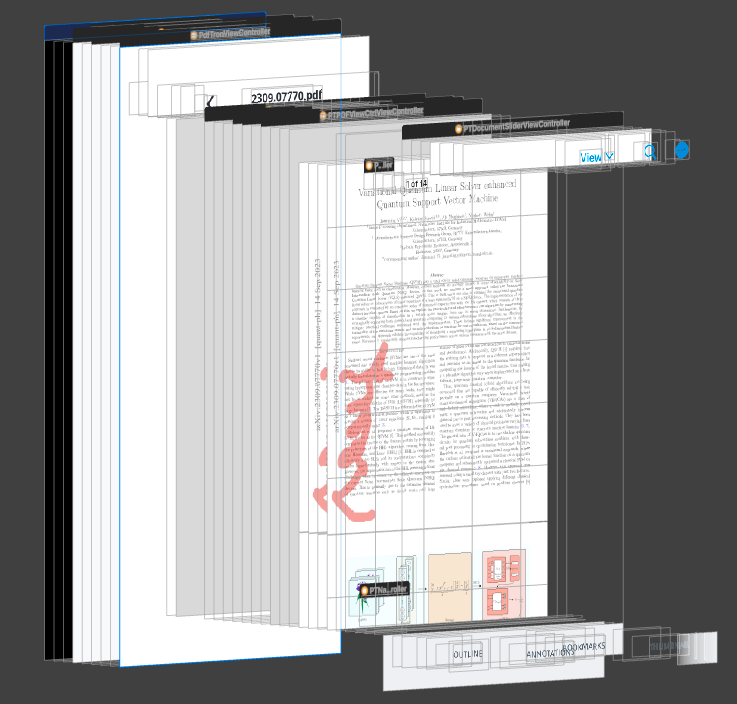
\includegraphics[width=0.8\textwidth]{Images/SideViewPdfViewController.png}
    \caption{PdfTronViewController dekompozicija}
    \label{img:pdfViewController}
\end{figure}
\newpage
\subsection{Anotacijų sąrašo PDF dokumente komponentas}
\enquote{PdfViewController} pavaizduoja dokumente esančias anotacijas, kurias galima redaguoti, ištrinti ar pridėti naujas.
 Taip pat yra galimybė pasirinkti anotacijos spalvą, dydį ir stilių. Esant dideliam anotacijų skaičiui, \enquote{AnnotationListViewController} pateikia anotacijų sąrašą, kurį galima filtruoti pagal anotacijos tipą, puslapį.
 Anotacijų sąraše galima pasirinkti anotaciją, kurią norima redaguoti, ištrinti ar peržiūrėti jos turinį ar sukurti naują formą. 
\begin{figure}[htbp!]
    \centering
    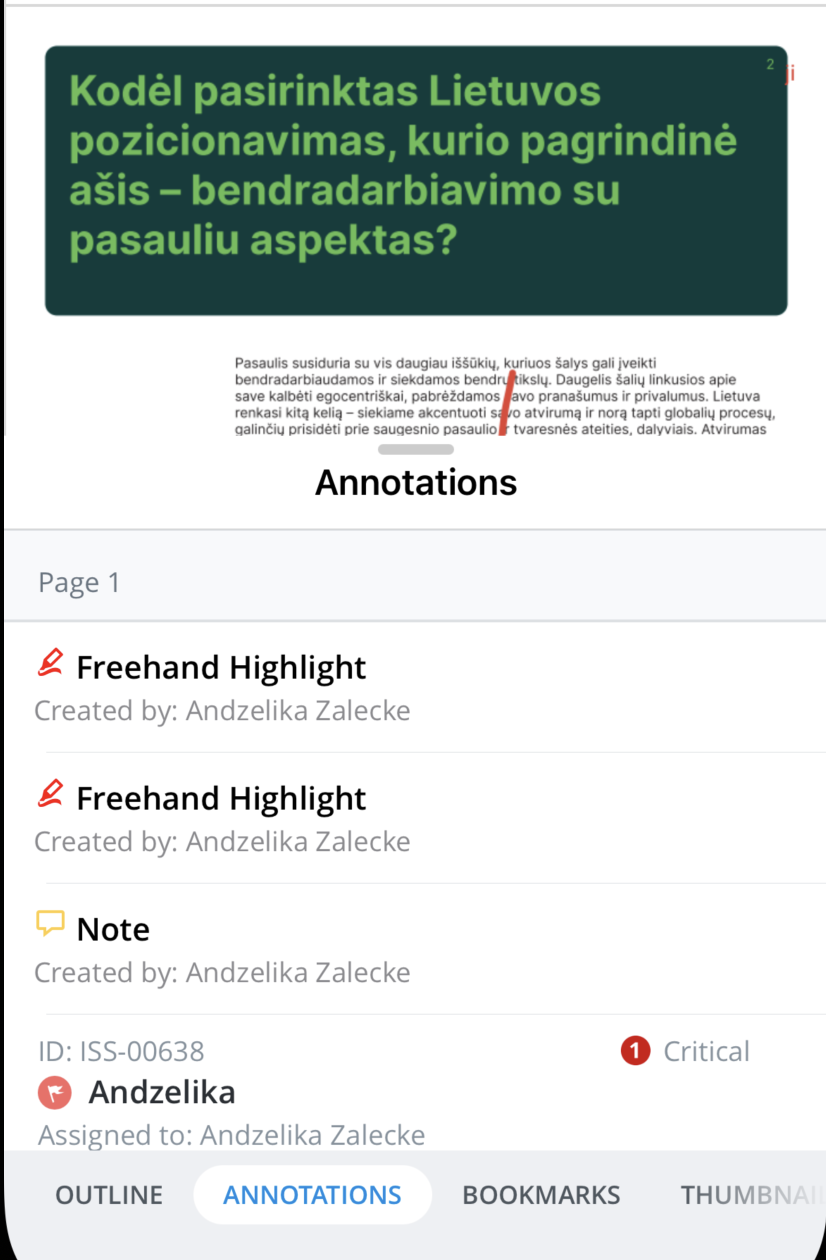
\includegraphics[width=0.6\textwidth]{Images/annotationList.png}
    \caption{Anotacijų sąrašo komponentas}
    \label{img:annotationList}
\end{figure}
\newpage
\subsection{Mobiliojoje programėlėje naudojamų mygtukų langas}
Projekte yra itin daug, įvairaus stiliaus mygtukų, atnaujinus iOS versiją ar programavimo karkasą, sunku pastebėti ar įvyko vizualūs pokyčiai. Tam buvo sukurtas Projekto mygtukų langas, kuriame galima matyti visus skirtingus, mygtukus programėlėje. 
Galima testuoti, kaip mygtukai reaguoja į įvairius veiksmus, kaip veikia jų animacijos, ar jie veikia pagal numatytą funkcionalumą. Visi mygtukai yra išdėstyti vienoje eilėje, todėl galima lengvai palyginti jų dydį, spalvą, formą ir kitas savybes. Mygtukų stiliaus nustatymas atnaujintas naudojant \enquote{UIButton.Configuration}, kuris leidžia paprastai, vienoje vietoje nustatyti specifinio mygtuko stilių. Senesni mygtukų stiliaus nustatymai buvo Storyboards, Swift kode.
Senesnis stiliaus nustatymo būdas turėjo problemų, nes ne visada buvo aišku, kur yra nustatymai, kurie nustato mygtuko stilių ir ar jie veikia. Naujasis būdas yra aiškesnis, nes visi nustatymai yra vienoje vietoje, lengvai prieinami ir aiškiai nurodyti.
\begin{figure}[htbp!]
    \centering
    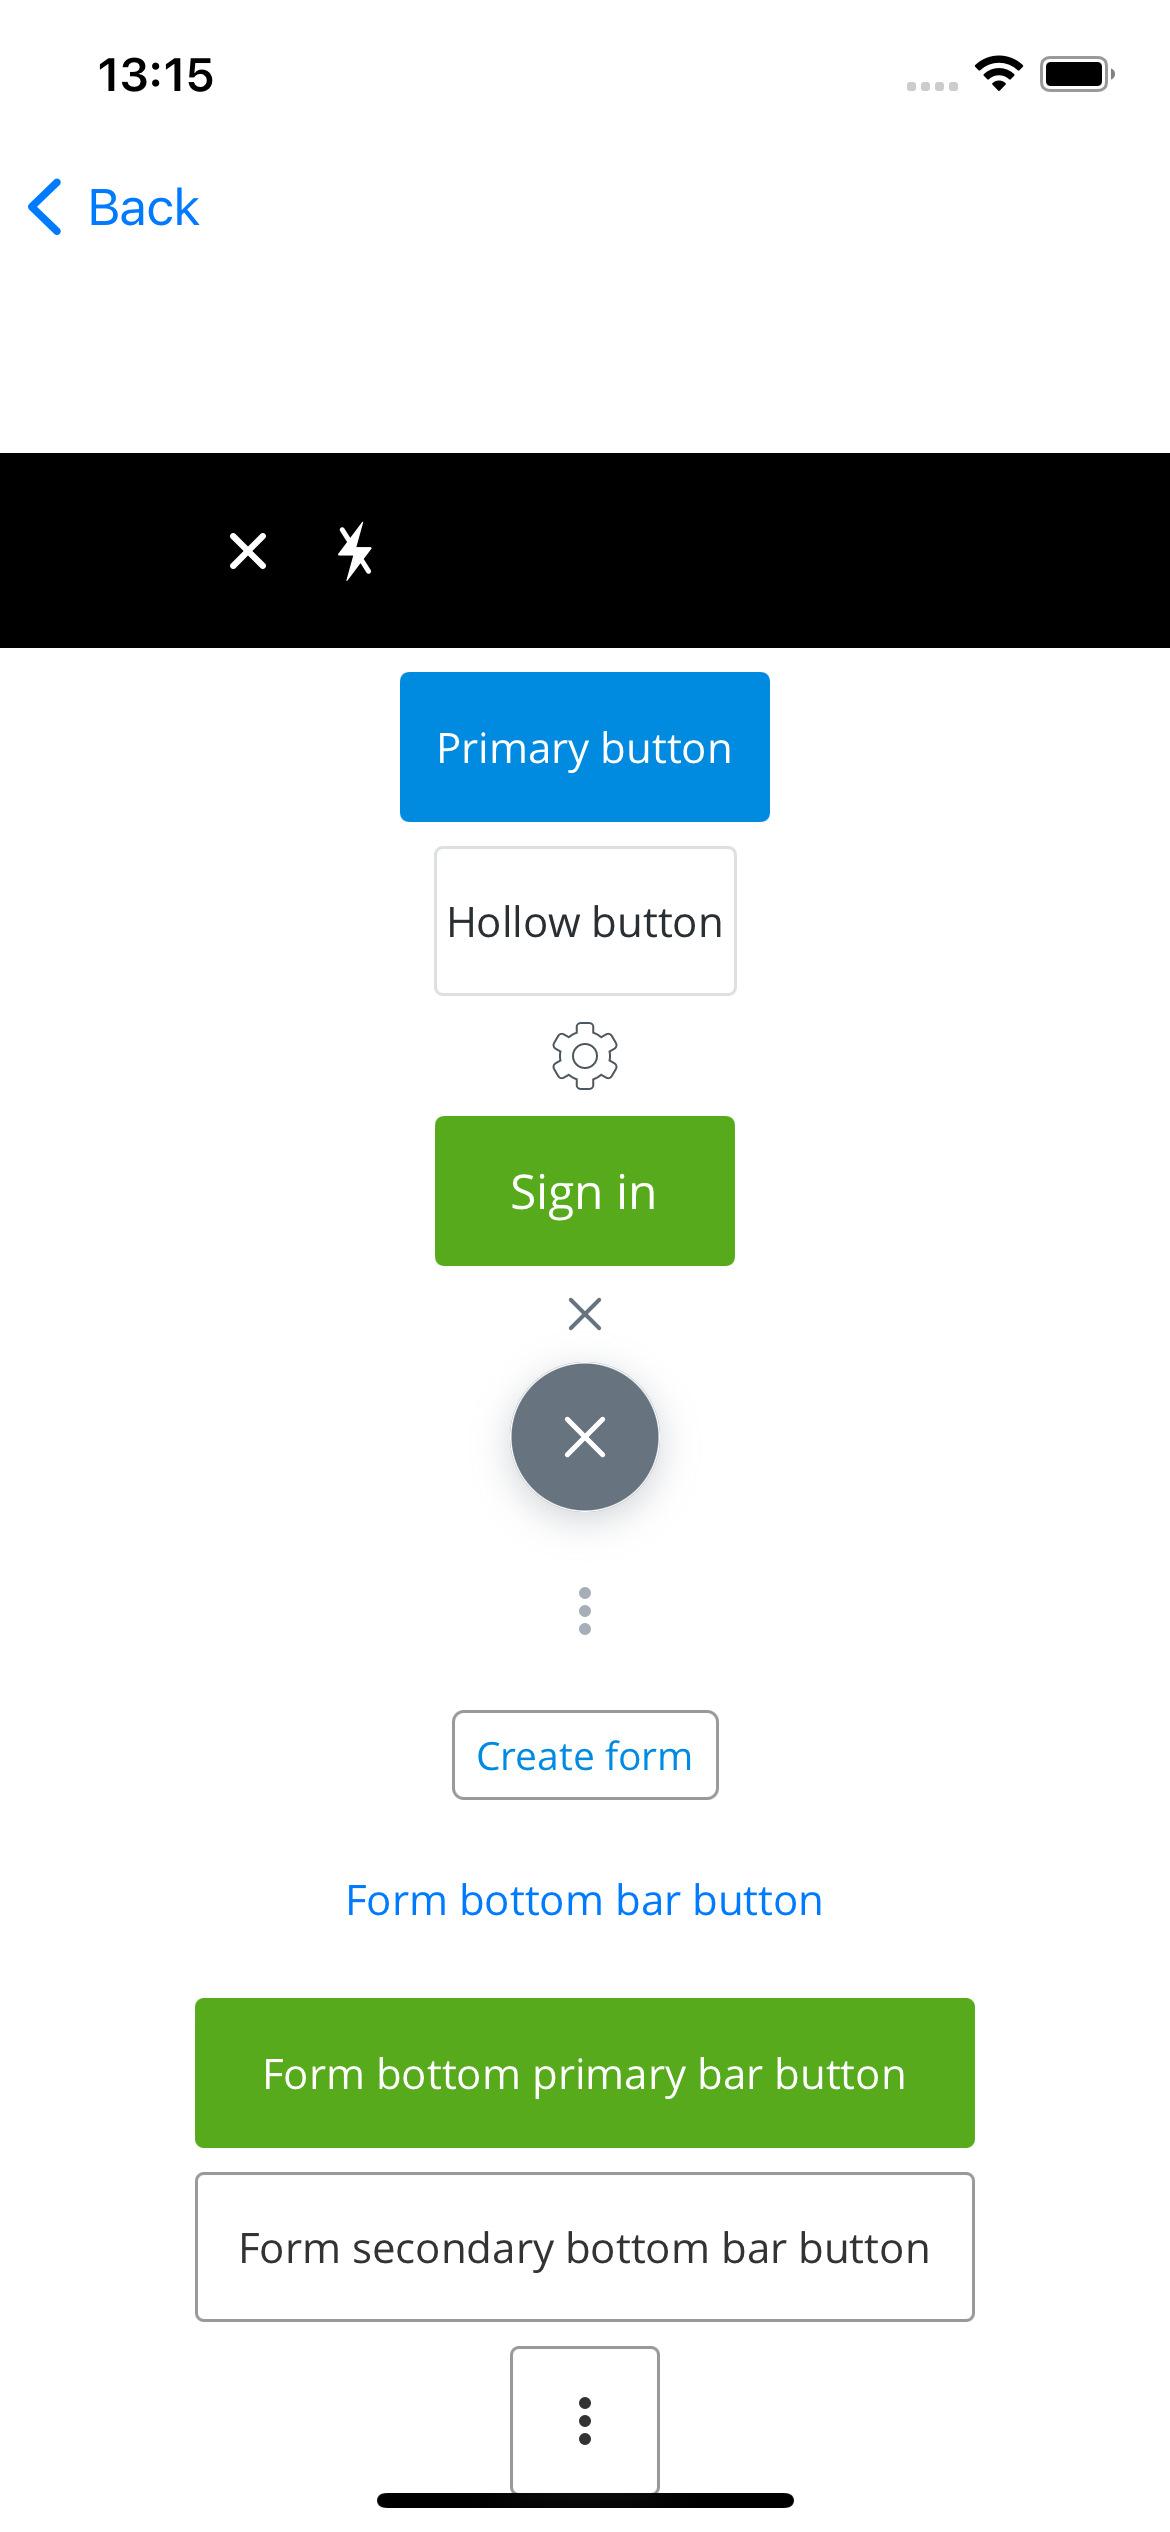
\includegraphics[width=0.4\textwidth]{Images/buttonsView.png}
    \caption{Projekto mygtukų langas}
    \label{fig:buttonsView.png}
\end{figure}
\newpage
\subsection{Vartotojo sąsajos komponentų programavimas naudojantis Jetpack compose karkasu}
Kadangi nuo 32 Android SDK versijos, Android pateikiamų iššokančių žinučių negalima keisti, nes tai turi tam tikrų saugumo spragų, buvo sukurtas naujas komponentas, pagal vartotojo sąsajos 
dizaino maketus. Jetpack Compose lengvai, net nepaleidus komponento įrenginyje, leidžia kurti vartotojo sąsajas, kurios atitinka naujausius dizaino standartus. Kiekvienas komponento pakeitimas iškart vizualiai matomas.
 Galima vizualiai pateikti vieno komponento visus testinius atvejus: Kai tekstas yra kelių eilučių, per ilgas ir pan. Taip pat galima pateikti, kaip komponentas elgiasi, kai jis yra įtrauktas į kitą komponentą.
  Yra galimybė sukurti įvairių dydžių ekranus, stebėti, kaip komponentas elgiasi, kiekvienu atveju. 

\begin{figure}[htbp!]
    \centering
    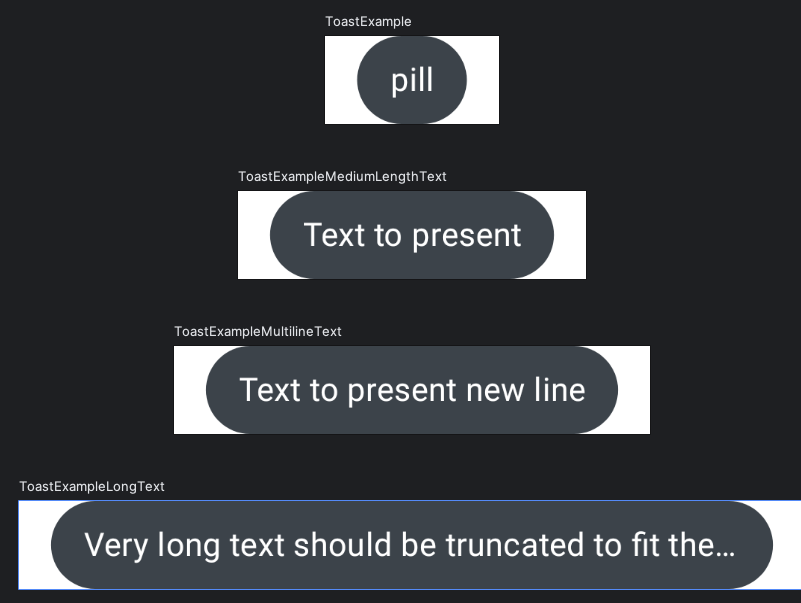
\includegraphics[width=0.7\textwidth]{Images/pillAndroid.png}
    \caption{Iššokančios žinutės komponentas}
    \label{fig:pill}
\end{figure}
\newpage
\subsection{Mobilioji programėlė su keleta pagrindinių langų}
Synchro Field mobilioji programėlė yra fragmentais grįsta su 2 pagrindiniais langais (\emph{angl. activities}). Toks dizaino sprendimas priimtas, nes virtualaus dvynio (\emph{angl. digital twin}) langas sukurtas kitos komandos. Šis komponentas yra
internetinio puslapio pobūdžio ir nėra tiesiogiai pritaikytas naudoti mobiliojoje programėlėje. Lengviausias būdas atvaizduoti, buvo sukurti atskirą pagrindinį langą, atlikti reikiamus pakeitimus ir atvaizduoti jį programėlėje.
 
 Norint pridėti iššokančios žinutės komponentą į 
programėlę, reikia sukurti ir pridėti komponentą į kiekvieną pagrindinį langą. Naudojamas tas pats viewModel objektas, kuris yra bendras visoms programėlės ekranams, norint, kad
iššokančių žinučių eilė būtų matoma visuose programėlės languose. 
\begin{figure}[htbp!]
    \centering
    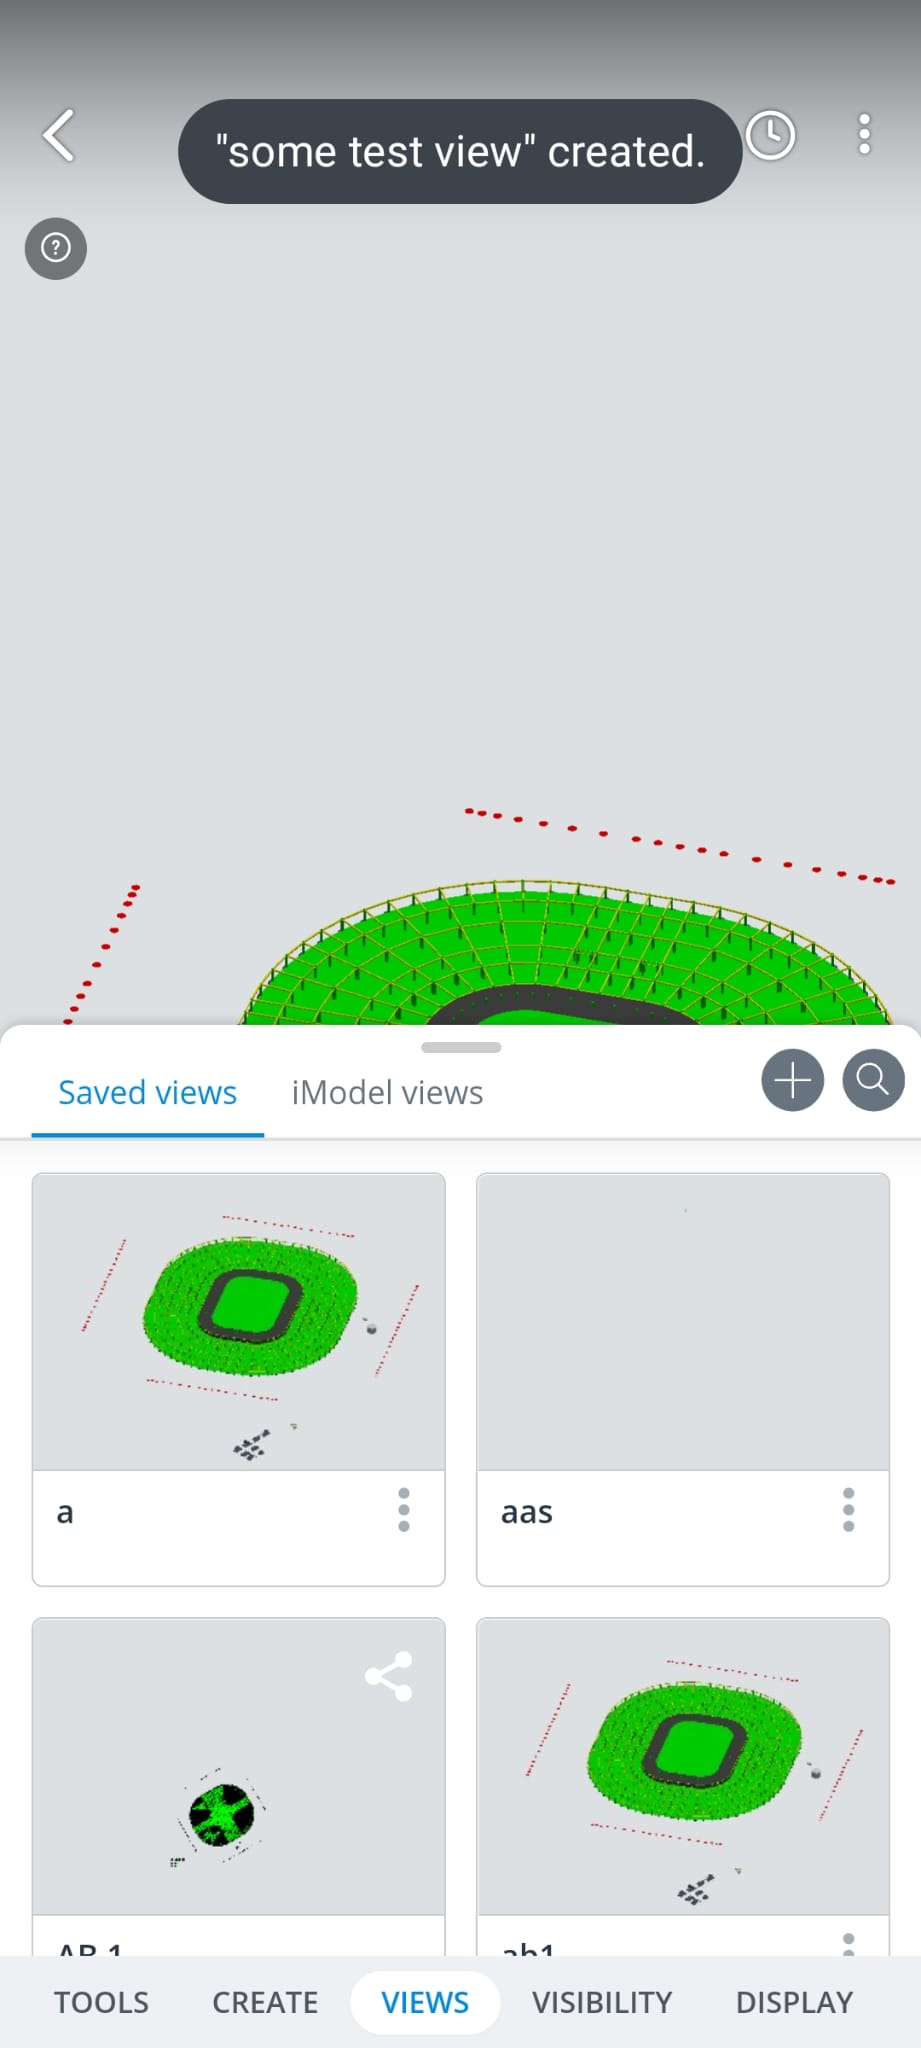
\includegraphics[width=0.45\textwidth]{Images/toastView.jpeg}
    \caption{Iššokančios žinutės komponento pavyzdys programėlėje}
    \label{fig:modelToastView}
\end{figure}
\end{document}